\chapter{Lineare Bauteile}

\section{Kondensator}
Ein Kondensator ist ein \textbf{passives Bauelement} und dazu, Energie zu speichern. Durch hineinfließenden \textbf{Strom}, wird Ladung in den Kondensator transportiert, wodurch \textbf{Spannung aufgebaut wird}.\\

\begin{center}
\begin{circuitikz}
        % Capacitor
        \draw(0,0) to[C] (2,0);

        % Voltages
        \draw[->, thick, blue] (0.5,0.5) -- (1.5,0.5) node[above left, blue] {$U_C$};
        
        % Currents
        \node[currarrow, red] at (0.25,0) {} node[above, red] {$I_C$};
\end{circuitikz}
\end{center}

Es gilt:
\begin{align}
    \Delta Q=C\cdot \Delta U=I\cdot \Delta t
\end{align}

\begin{itemize}
    \item \textbf{$\Delta Q$}... Ladungsänderung in \textbf{Coulomb ($C$)}
    \item \textbf{$C$}... Kapazität in \textbf{Farad ($F$)}
    \item \textbf{$\Delta t$}... Zeitänderung in \textbf{Ampere ($A$)}
    \item \textbf{$\Delta U$}... Spannungsänderung in \textbf{Volt ($V$)}
\end{itemize}

\newpage

\subsection{Schaltung von Kondensatoren}
\subsubsection*{Serienschaltung}
Es gilt:
\begin{align}
    C_g&=\frac{C_1\cdot C_2}{C_1+C_2} \\
    \frac{1}{C_g}&=\frac{1}{C_1}+\frac{1}{C_2}
\end{align}
\begin{center}
\begin{circuitikz}
        % Capacitor
        \draw(0,0) to[C=$C_1$] (2,0) to[C=$C_2$] (4,0);

        % Voltages
        \draw[->, thick, blue] (0.5,-1) -- (1.5,-1) node[below left, blue] {$U_{C_1}$};
        \draw[->, thick, blue] (2.5,-1) -- (3.5,-1) node[below left, blue] {$U_{C_2}$};
        
        % Currents
        \node[currarrow, red] at (0.25,0) {} node[below, red] {$I_{C_g}$};
\end{circuitikz}
\end{center}

\subsubsection*{Parallelschaltung}
Es gilt:
\begin{align}
    C_g&=C_1+C_2
\end{align}
\begin{center}
\begin{circuitikz}
        % Capacitor
        \draw(0,0) to[C=$C_1$] (2,0);
        \draw(0,-2) to[C=$C_2$] (2,-2);

        % Wires
        \draw[black] (0,0) -- (0,-2);
        \draw[black] (2,0) -- (2,-2);
        \draw[black] (0,-1) -- (-1,-1);
        \draw[black] (2,-1) -- (3,-1);

        % Voltages
        \draw[->, thick, blue] (0.5,-3) -- (1.5,-3) node[below left, blue] {$U_{C_g}$};
        
        % Currents
        \node[currarrow, red] at (0.25,0) {} node[above, red] {$I_{C_1}$};
        \node[currarrow, red] at (0.25,-2) {} node[below, red] at (0.25,-2) {$I_{C_2}$};
\end{circuitikz}
\end{center}

\newpage

\subsubsection*{Beispiel}
Gegeben:
\begin{center}
\begin{circuitikz}
        % Capacitor
        \draw(0,0) to[C=$C_1$] (0,-2) node[left] at (-0.5,-1) {$100nF$};
        \draw(-1,-2) to[C=$C_2$,left] (-1,-4);
        \draw(1,-2) to[C=$C_3$] (1,-4);

        % Wires
        \draw[black] (-1,-2) -- (1,-2);
        \draw[black] (-1,-4) -- (1,-4);
        \draw[black] (0,-4) -- (0,-5);
        
        % Voltages
        \draw[->, thick, blue] (2.5,-2) -- (2.5,-4) node[above right, blue] {$U_{C_3}=3V$};
        
        % Currents
        % \node[currarrow, red] at (0.25,0) {} node[above, red] {$I_{C_1}$};
        % \node[currarrow, red] at (0.25,-2) {} node[below, red] at (0.25,-2) {$I_{C_2}$};
\end{circuitikz}
\end{center}

Gesucht: $Q_1, Q_2, Q_3, U_{C_1}, U_{C_2}, U_{C_3}, C_g$

\begin{align}
    Q_2&=C_2\cdot U_{C_2}=1[\mu F]\cdot 3[V]=3[\mu C] \\
    Q_3&=C_3\cdot U_{C_3}=2[\mu F]\cdot 3[V]=6[\mu C] \\
    Q_1&=Q_2+Q_3=3[\mu C]+6[\mu C]=9[\mu C]
\end{align}
\begin{align}
    \Rightarrow U_{C_1}&=\frac{Q_1}{C_1}=\frac{9[\mu C]}{0,1[\mu F]=90[V]}
\end{align}
\begin{align}
    C_{2,3}&=C_2+C_3=1[\mu F]+2[\mu F]=3[\mu F]\\
    C_g&=\frac{C_{2,3}\cdot C_1}{C_{2,3}+ C_1}=\frac{3[\mu F]\cdot 100[nF]}{3[\mu F]+ 100[nF]} \\
    C_g&\approx 96,774[nF]
\end{align}
\begin{align}
    U_g=\frac{Q_g}{C_g}=\frac{9[\mu C]}{96,774[nF]}=93[V]
\end{align}

\newpage

\subsection{Lade- \& Entladekurven}
Bei einem idealen Kondensator, d.h. mit einem Innenwiderstand von $0 \Omega$, lädt sich dieser mit einer linearen Funktion auf. Ebenso würde er sich linear entladen, würde eine negative Spannung angelegt werden.

\begin{center}
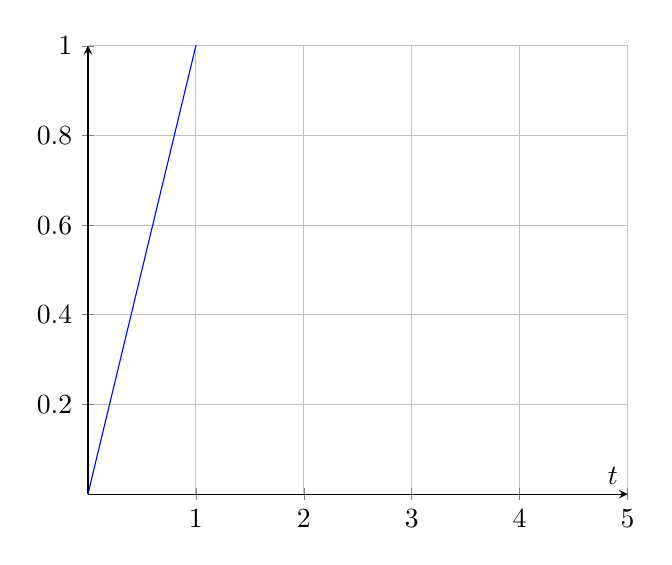
\begin{tikzpicture}
\begin{axis} [
        grid=both,
        xmin=0, xmax=5,
        ymin=0, ymax=1,
        xlabel=$t$,
        axis lines=middle,
        % restrict x to domain=0:5,
        % restrict y to domain=0:1
    ]
    
    \addplot[blue] {x} node[right] {$u(t)$};
    % \addplot[red] {1} {$i(t)$};

\end{axis}
\end{tikzpicture}
\end{center}

Reale Kondensatoren besitzen jedoch einen Innenwiderstand $R_i > 0 \Omega$ und laden bzw. entladen sich deswegen mit einer Exponentialfunktion.

\begin{center}
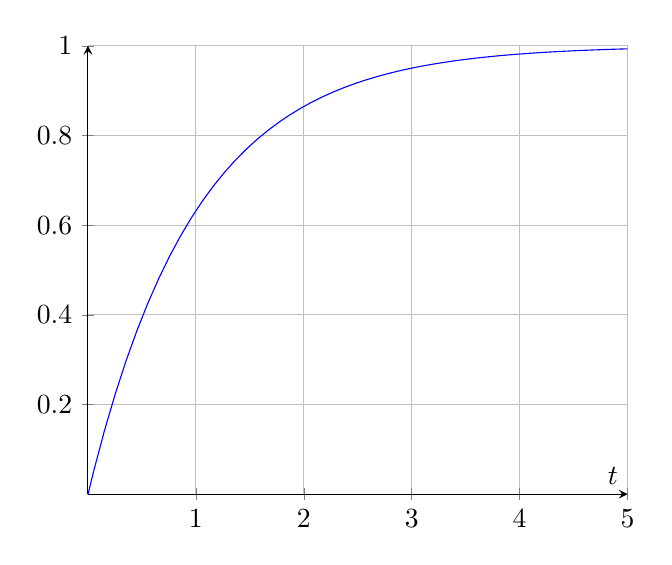
\begin{tikzpicture}
\begin{axis} [
        grid=both,
        xmin=0, xmax=5,
        ymin=0, ymax=1,
        xlabel=$t$,
        axis lines=middle,
        restrict x to domain=-1:6,
        restrict y to domain=-1:2
    ]
    \addplot[blue, samples=100] {1-exp(-x)};

    % \draw[black]
    % \addplot[black, samples=2] {x} node[left] {$\tau$};
    % \addplot[black, dashed, samples=2] {y};
\end{axis}
\end{tikzpicture}
\end{center}

\newpage

\subsection{Tau-Messung}



\subsection{Blindwiderstand}
Der Blindwiderstand eines Kondensators wird mit $\underline{x}_C=\frac{1}{j\omega C}$ beschrieben. Das heißt, die Impedanz (der "Widerstand") ist abhängig von der Frequenz ($j\omega$).
\begin{itemize}
    \item Bei niedrigen Frequenzen wird der Kondensator zum Leerlauf:\\
    $\omega \rightarrow 0: \frac{1}{j\omega C} = \frac{1}{0} = \infty$

    \item Bei hohen Frequenzen wird der Kondensator zum Kurzschluss:\\
    $\omega \rightarrow \infty: \frac{1}{j\omega C} = \frac{1}{\infty} = 0$
\end{itemize}

\newpage

\section{Spule}
Eine Spule ist ein \textbf{passives Bauelement} um \textbf{Energe zu speichern} in dem es ein \text{Magnetfeld erzeugt}. Außerdem ist sie \textbf{frequenzabhängig}. 

\subsubsection*{Anwendungen}
\begin{itemize}
    \item Filter
    \item Schwingkreise
    \item Energiespeicher
    \item Störunterdrückung (Stromflussglättung)
\end{itemize}

\subsubsection*{Wichtige Formeln}
\begin{table}[!htb]
    \centering
    \begin{tabular}{|c|c|}
        \hline
        Linearer Stromanstieg/-abfall & $L\cdot \Delta i = U_L \cdot \Delta t$ \\
        Impedanz (komplexer Widerstand) & $x_L = j\omega L = j2\pi fL$ \\
        Wechselstromverhalten & $u(t) = L\cdot \frac{di(t)}{dt}$ \\
        Serienschaltung zweier magnetisch nicht gekoppelter Spulen& $L_{g}=L_1+L_2$ \\
        Parallelschaltung zweier magnetisch nicht gekoppelter Spulen& $L_{g}=\frac{L_1\cdot L_2}{L_1+ L_2}$ \\
        \hline
    \end{tabular}
    \caption{Wichtige Formeln}
\end{table}

\subsection{Lade- \& Entladekurven}

\subsection{Zeigerdiagramm}

\newpage

\section{Induktivitäten}
\subsection{Definition der Induktivität $L$ einer Spule}
Die Induktivität einer Spule beschreibt die Proportionalität zwischen magnetischem Verkettungsfluss $\Phi_v$, und Spulenstrom $i$.
\begin{align}
    \Phi_v=N\cdot \Phi = L \cdot i
\end{align}
\begin{itemize}
    \item $\Phi$ ... Fluss durch die Spule in [$Wb$]
    \item $N$ ... Windungszahl
    \item $\Phi_v$ ... Verkettungsfluss der Spule in [$Wb$]
    \item $L$ ... Induktivität in [$H$]
    \item $i$ ... Strom durch die Spule [$A$]
\end{itemize}

\subsection{Selbstinduktionsspannung einer Spule}
\begin{align}
    u_L = -L \cdot \frac{\Delta i}{\Delta t}
\end{align}
\begin{itemize}
    \item $u_L$ ... Selbstinduktionsspannung in [$V$]
    \item $L$ ... Induktivität in [$H$]
    \item $\frac{\Delta i}{\Delta t}$ ... Stromänderung in [$\frac{A}{s}$]
\end{itemize}

\subsection{Induktivität einer Spule}
Die Induktivität einer Spule ist proportional dem Qudrat der Windungszahl.
\begin{align}
    L=N^2\cdot \frac{1}{R_m}=N^2\cdot \Lambda
\end{align}
\begin{itemize}
    \item $L$ ... Induktivität in [$H$]
    \item $N$ ... Windungszahl
    \item $R_m$ ... magnetischer Widerstand in [$\frac{1}{H}$]
    \item $\Lambda$ ... magnetischer Leitwert in [$H$]
\end{itemize}

\subsection{Induktivität einer schlanken Zylinderspule}
\begin{align}
    L=N^2\cdot\mu_0\cdot \frac{A}{l}
\end{align}
\begin{itemize}
    \item $L$ ... Induktivität in [$H$]
    \item $N$ ... Windungszahl
    \item $\mu_0$ ... Permeabilität des leeren Raumes in [$\frac{Vs}{Am}$]
    \item $R_m$ ... Spulenfläche in [$m^2$]
    \item $l$ ... Spulenlänge in [$m$]
\end{itemize}

\subsection{Induktivität einer Zylinderspule mit $\frac{l}{d}>10$}
\begin{align}
    L=k\cdot N^2 \mu_0 \cdot \frac{A}{l}
\end{align}
\begin{itemize}
    \item $L$ ... Induktivität in [$H$]
    \item $N$ ... Windungszahl
    \item $k$ ... Korrekturfaktor
    \item $\mu_0$ ... Permeabilität des leeren Raumes in [$\frac{Vs}{Am}$]
    \item $A$ ... Spulenfläche in [$m^2$]
    \item $l$ ... Spulenlänge in [$m$]
\end{itemize}

\subsection{Induktivität einer schlanken Zylinderspule mit Eisenkern}
\begin{align}
    L=N^2\cdot\mu_0\cdot\mu_r\cdot \frac{A}{l_{Fe}}
\end{align}
\begin{itemize}
    \item $L$ ... Induktivität in [$H$]
    \item $N$ ... Windungszahl
    \item $\mu_0$ ... Permeabilität des leeren Raumes in [$\frac{Vs}{Am}$]
    \item $\mu_0$ ... relative Permeabilität im Arbeitspunkt
    \item $R_m$ ... Spulenfläche in [$m^2$]
    \item $l_{Fe}$ ... mittlere Eisenlänge [$m$]
\end{itemize}

\newpage

\section{Transformator \& Übertrager}
Zwei oder mehrere magnetisch gekoppelte Spulen:
\todo{Insert Picture}

\subsection{Transformator}

\subsection{Übertrager}

\subsubsection*{Übersetzungsverhältnis}

Bei einem Transformator werden die Spannungen im Verhältnis der Windungszahlen von Primär- und Sekundärspule umgesetzt. Die Ströme werden im umgekehrten Verhältnis der Windungszahlen transformiert.

\begin{align}
    \text{ü} = \frac{U_1}{U_2} = \frac{I_1}{I_2} = \frac{N_1}{N_2}
\end{align}
\begin{itemize}
    \item ü ... Übersetzungsverhältnis
    \item $U_1$ ... Primärspannung in [$V$]
    \item $U_2$ ... Sekundärspannung in [$V$]
    \item $I_1$ ... Primärstrom in [$A$]
    \item $I_2$ ... Sekundärstrom in [$A$]
    \item $N_1$ ... Primärwindungen
    \item $N_2$ ... Sekundärwindungen
\end{itemize}

\newpage

\section{RLC Netzwerke}
\subsection{Die Zeitkonstante Tau}
Die Zeitkonstante $\tau$ (Tau) beschreibt den Zusammenhang zwischen den verbauten Bauteilen. Somit können mithilfe von Spannungskurven auf die Bauteilwerte rückgeschlossen werden. \\
Eine weitere Möglichkeit auf Tau zu kommen ist die Berechnung mit den unten angegebenen Formeln:
\begin{itemize}
    \item RC-Netzwerk: {\large $\tau = R\cdot C$}
    \item LR-Netzwerk: {\large $\tau = \frac{L}{R}$}
\end{itemize}
\subsubsection{Taumessung bei Ladekurven}
$\tau$ kann sowohl beim Entladevorgang (siehe „Taumessung bei Entladekurven“) als auch beim Ladevorgang abgelesen werden. Bei Ladevorgängen wird eine Tangente aus dem Ursprung der Funktion gelegt. Diese Tangente schneidet anschließend den Maximalspannungswert. Wenn man diesen Schnittpunkt dann im 90° Winkel zur Zeitachse runter verbindet, kann Tau an diesem Punkt abgelesen werden:
\subsubsection*{RC-Glied}
\begin{center}
\begin{circuitikz}
    \draw (0,0) to[R=$R$] (2,0);
    \draw (2,0) to[C=$C$] (2,-1.5);
    \draw (0,-1.5) -- (3,-1.5);
    \draw (2,0) -- (3,0);
    \draw[->,blue,>=latex,fill=blue] (0,-0.25) -- (0,-1.25) node[midway, left,blue] {${U}_e$};
    \draw[->,blue,>=latex,fill=blue] (3,-0.25) -- (3,-1.25) node[midway, right,blue] {${U}_a$};
    \draw[black,fill=black] (2,0) circle (1.5pt);
    \draw[black,fill=black] (2,-1.5) circle (1.5pt);
    \draw[black] (0,0) circle (1.5pt);
    \draw[black] (0,-1.5) circle (1.5pt);
    \draw[black] (3,0) circle (1.5pt);
    \draw[black] (3,-1.5) circle (1.5pt);
\end{circuitikz}
\end{center}

\begin{center}
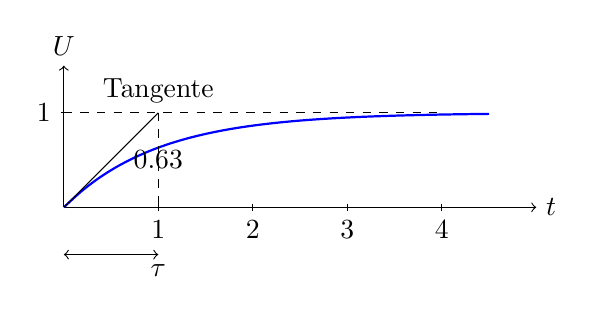
\begin{tikzpicture}[scale=1.2]
    % Achsen
    \draw[->] (0,0) -- (5,0) node[right] {$t$};
    \draw[->] (0,0) -- (0,1.5) node[above] {$U$};
    
    % Kurve
    \draw[thick, domain=0:4.5, smooth, variable=\x, blue] plot ({\x}, {1-exp(-\x)});
    
    % Beschriftungen
    \draw[dashed] (0,1) node[below] {} -- (4,1);
    \draw (0,0) -- (1,1) node[above] {Tangente};
    \draw[<->] (0,-0.5) -- (1,-0.5) node[below] {$\tau$};
    \draw[dashed] (1,1) -- (1,0) node[midway]{$0.63$};
    
    % Achsenbeschriftungen
    \foreach \x in {1,2,3,4}
        \draw (\x cm,1pt) -- (\x cm,-1pt) node[anchor=north] {$\x$};
    \foreach \y in {1}
        \draw (1pt,\y cm) -- (-1pt,\y cm) node[anchor=east] {$\y$};
        
\end{tikzpicture}
\end{center}
Wichtige Kenndaten zu Tau bei Entladekurven:
\begin{itemize}
    \item Bei 63\% der Maximalspannung kann $\tau$ abgelesen werden.
    \item Bei 95\% der Maximalspannung kann $2\tau$ abgelesen werden.
    \item Bei 99\% der Maximalspannung kann $3\tau$ abgelesen werden
\end{itemize}
\subsubsection{Taumessung bei Entladekurven}
Im folgenden Bild ist die Spannung an einer Spule angegeben. $\tau$ befindet sich bei 37$\%$ der Maximalspannung $U_0$. Nach dem Einzeichnen der 37\% kann $\tau$ auf der Zeitachse abgelesen werden:
%--------------------------
%   kommt noch was rein :3
%--------------------------
Wichtige Kenndaten zu Tau bei Entladekurven:
\begin{itemize}
    \item Bei 37$\%$ der Maximalspannung (nach 63$\%$ Abfall) kann $\tau$ abgelesen werden.
    \item Bei 5$\%$ der Maximalspannung (nach 95$\%$ Abfall) kann $2\cdot\tau$ abgelesen werden.
    \item Bei 1$\%$ der Maximalspannung (nach 99$\%$ Abfall) kann $3\cdot\tau$ abgelesen werden.
\end{itemize}
\subsection{Schwingkreis}
Ein elektrischer Schwingkreis (auch als Resonanzkreis bekannt) ist eine resonanzfähige elektrische Schaltung aus einer Spule $L$ und einem Kondensator $C$, die elektrische Schwingungen ausführen kann. In der Mechanik gibt es ebenfalls Schwingkreise. Diese sind aber für diese Mitschrift nicht von Bedeutung. Ein durchwegs bekanntes mechanisches Bauteil, welches elektrische Schwingungen erzeugen kann, ist der Quarz.

\subsubsection{LC-Schwingkreis}
Ein sogenannter $LC$-Schwingkreis besteht wie der Namen schon sagt aus einer Spule und einem Kondensator. Zusätzlich wird ein Widerstand eingebaut, dass der Schwingkreis ordentlich schwingen kann.
\begin{center}
	\begin{circuitikz}
        \draw (0,0) to[C=$C$] (0,-2);
        \draw (2,0) to[L=$L$] (2,-2);

        \draw (0,0) -- (2,0);
        \draw (0,-2) -- (2,-2);
	\end{circuitikz}
\end{center}
Um die Resonanzfrequenz oder auch umgangssprachlich Schwingfrequenz genannt, kann über die sogenannte „Thomson'sche Schwingungsformel“ berechnet werden:
\begin{center}
    \begin{Large}
    $f_{r} = \frac{1}{2 \cdot \pi \cdot \sqrt{L \cdot C}}$
    \end{Large}
\end{center}
Die Kreisfrequenz bei Resonanz wird mit der folgenden Formel berechnet:
\begin{center}
    \begin{Large}
    $\omega_{r} = \frac{1}{\sqrt{L \cdot C}}$
    \end{Large}
\end{center}
Die untere und die obere Grenzfrequenz ergeben sich aus den $-3dB$-Punkten ($3dB$-Bandgrenzen). Bei $\sqrt{2}$ der Maximalspannung können die Grenzfrequenzen berechnet werden. Ein anderer Weg auf die Bandgrenzen zu kommen ist es, drei dB von der Resonanzfrequenz abzuziehen und diese dann einzuzeichnen.
%--------------------------
%   kommt noch was rein :3
%--------------------------

\begin{center}
    \begin{Large}
    $B = f_{o} - f_{u}$     \\[10pt] 
    $B = \frac{f_{r}}{Q}$
    \end{Large}
\end{center}
\begin{itemize}
    \item B ... Bandbreite in Hz
    \item $f_{o}$ ... obere Grenzfrequenz in Hz
    \item $f_{u}$ ... untere Grenzfrequenz in Hz
    \item $f_{r}$ ... Resonanzfrequenz in Hz
    \item Q ... Güte des Resonanzkreises
\end{itemize}


\subsubsection*{Parallelschwingkreis}
\begin{center}
\begin{circuitikz}
    \draw (3,-1) to[R=$R$] (3,-3);
    \draw (7,-1) to[C=$C$] (7,-3);
    \draw (5,0) to[L=$L$] (5,-4);

    \draw (0,0) -- (0,-1.5);
    \draw (0,-4) -- (0,-2.5);
    \draw (0,0) -- (5,0);
    \draw (0,-4) -- (5,-4);
    \draw (3,-1) -- (7,-1);
    \draw (3,-3) -- (7,-3);

    \draw[black] (0,-1.55) circle (2pt);
    \draw[black] (0,-2.45) circle (2pt);
    \draw[black,fill=black] (5,-1) circle (1.5pt);
    \draw[black,fill=black] (5,-3) circle (1.5pt); 

    \draw (-0.5,-2) .. controls (-0.25,-2.15) .. (0,-2);
    \draw (0,-2) .. controls (0.25,-1.85) .. (0.5,-2);
\end{circuitikz}

\end{center}
\begin{center}
    \begin{Large}
    $Q = \frac{R}{X} = \frac{R}{2 \cdot \pi \cdot f_{r} \cdot L} =$ \\[10pt]
    $2 \cdot \pi \cdot f_{r} \cdot C \cdot R =$ \\[10pt]
    $R \cdot \sqrt{\frac{C}{L}} $
    \end{Large}
\end{center}
%--------------------------
%   kommt noch was rein :3
%--------------------------
Bei diesem Diagramm eilt die Spannung dem Strom hinterher.

\subsubsection*{Serienschwingkreis}
\begin{center}
\begin{circuitikz}
    \draw (0,0) to[R=$R$] (2,0);
    \draw (2,0) to[L=$L$] (4,0);
    \draw (4,0) to[C=$C$] (6,0);

    \draw (0,0) -- (0,-2);
    \draw (6,0) -- (6,-2);
    \draw (0,-2) -- (2.5,-2);
    \draw (6,-2) -- (3.5,-2);

    \draw[black] (2.57,-2) circle (2pt);
    \draw[black] (3.43,-2) circle (2pt);


    \draw (2.75,-2) .. controls (2.875,-2.15) .. (3,-2);
    \draw (3,-2) .. controls (3.125,-1.85) .. (3.25,-2);

\end{circuitikz}
\end{center}
\begin{center}
    \begin{Large}
    $Q = \frac{X}{R} = \frac{2 \cdot \pi \cdot f_{r} \cdot L}{R} =$ \\[10pt]
    $\frac{1}{2 \cdot \pi \cdot f_{r} \cdot C \cdot R}  =$ \\[10pt]
    $\frac{1}{R} \cdot \sqrt{\frac{L}{C}} $
    \end{Large}
\end{center}
%--------------------------
%   kommt noch was rein :3
%--------------------------
Bei diesem Diagramm eilt der Strom der Spannung hinterher.

\subsubsection{Quarz - Schwingkreis}
Hier angegeben ist der Pierce Oszillator. Dieser kann einfach mit einem Quarz der Wahl aufgebaut werden. Es kann durchaus möglich sein, dass es bei Microcontrollern oder ICs nötig ist, einen Quarz-Oszillator aufzubauen.
\begin{center}
\begin{circuitikz}
    \draw (3,0) node[invschmitt]{} (4,0);
    \draw (1,0) node[american not port]{} (2,0);
    \draw (0,-2) to[R=$R1$] (2,-2);
    \draw (2,-2) to[R=$R2$] (2,-4);
    \draw (0,-4) to[C=$C1$] (0,-6);
    \draw (2,-4) to[C=$C2$] (2,-6);
    \draw (1,-4) node[piezoelectricshape]{} (2,-4);
    \draw (1,-6) node[rground]{};
    \draw (3.5,-2) node[rground]{};

    
    \draw (0,0) -- (0.5,0);
    \draw (0,0) -- (0,-4);
    \draw (0,-4) -- (0.7,-4);
    \draw (2,-4) -- (1.3,-4);
    \draw (2,0) -- (2,-2);
    \draw (0,-6) -- (2,-6);
    \draw (1.5,0) -- (2.5,0);
    \draw (3.5,-2) -- (3.7,-2);

    \draw[black] (3.8,0) circle (2pt);
    \draw[black] (3.8,-2) circle (2pt);
    \draw[black,fill=black] (2,0) circle (1.5pt);
    \draw[black,fill=black] (0,-2) circle (1.5pt);
    \draw[black,fill=black] (2,-2) circle (1.5pt);
    \draw[black,fill=black] (2,-4) circle (1.5pt);
    \draw[black,fill=black] (0,-4) circle (1.5pt);
    \draw[black,fill=black] (1,-6) circle (1.5pt);

    \draw[blue,>=latex,fill=blue] (4,-1.8) -- (4.4,-1.8);
    \draw[blue,>=latex,fill=blue] (4.4,-1.8) -- (4.4,-0.5);
    \draw[blue,>=latex,fill=blue] (4.4,-0.5) -- (4.8,-0.5);
    \draw[blue,>=latex,fill=blue] (4.8,-0.5) -- (4.8,-1.8);
    \draw[blue,>=latex,fill=blue] (4.8,-1.8) -- (5.2,-1.8);
    \draw[blue,>=latex,fill=blue] (5.2,-1.8) -- (5.2,-0.5);
    \draw[blue,>=latex,fill=blue] (5.2,-0.5) -- (5.6,-0.5);
    \draw[blue,>=latex,fill=blue] (5.6,-0.5) -- (5.6,-1.8);
    \draw[blue,>=latex,fill=blue] (5.6,-1.8) -- (6,-1.8);
    
\end{circuitikz}
\end{center}
In dieser Schaltung wurden beispielsweise folgende Bauteilwerte genutzt:
\begin{itemize}
    \item $R_{1}: 100 k\Omega ... 10 M\Omega$
    \item $R_{2}: 10 \Omega ... 4.7 k\Omega$
    \item $C_{1}, C_{2}: 10 pF ... 82 pF$
\end{itemize}

\subsection{RLC-Kombinationen}
\begin{center}
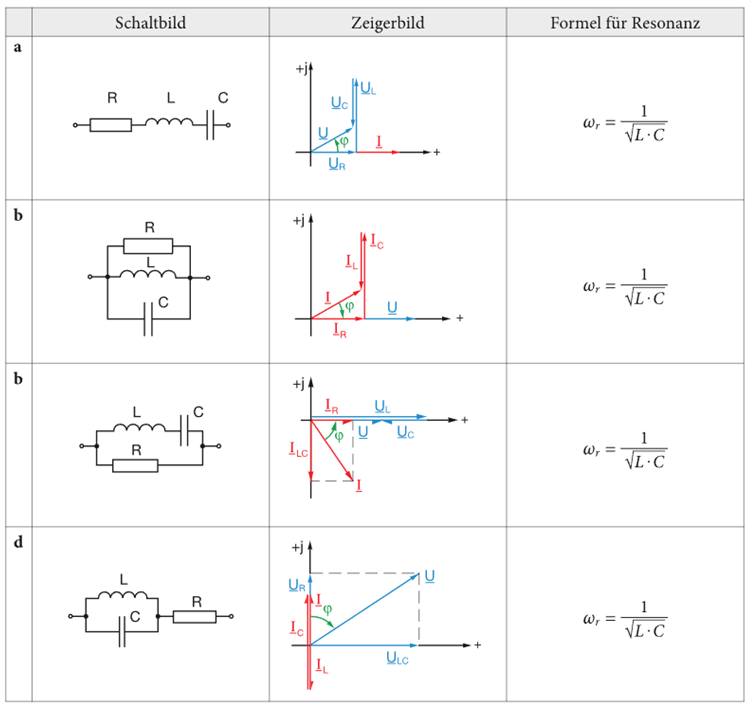
\includegraphics[width=.75\linewidth]{LineareBauteile/RLC-1.png}
\vspace{0.5cm} \\
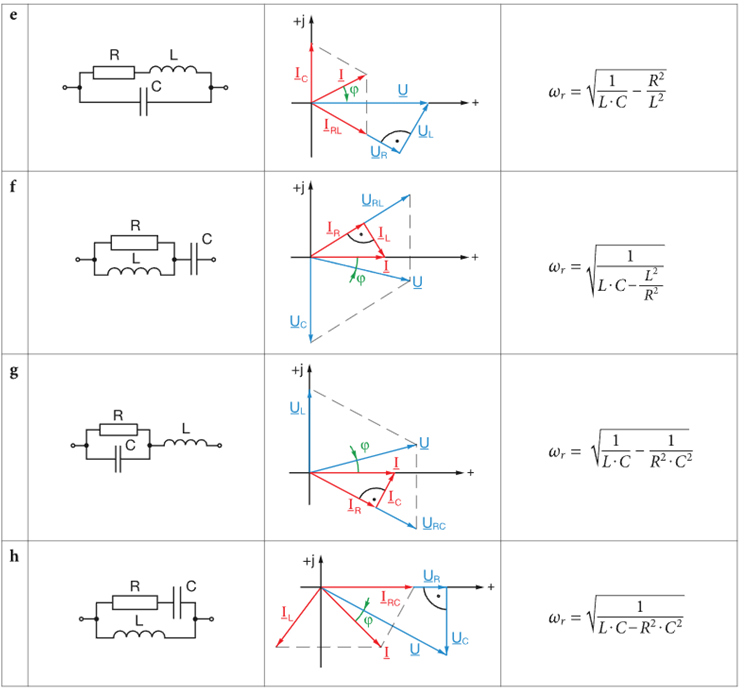
\includegraphics[width=.75\linewidth]{LineareBauteile/RLC-2.png}
\end{center}

\todo{Güte?}

% \newpage

% \section{Resonanzkreise}

% \subsection{Güte}

% \subsection{Bandbreite}

\newpage

\section{Übertragungsfunktion}
Die Übertragungsfunktion beschreibt das Ausgangs- im Vergleich zum
Eingangssignal und ist definiert als
\begin{align}
    \underline{H}(j\omega)=\frac{\underline{U}_2}{\underline{U}_1}=\frac{\underline{U}_a}{\underline{U}_e}
\end{align}
wobei $\underline{U}_1$, $\underline{U}_e$ der Eingang und $\underline{U}_2$, $\underline{U}_a$ der Ausgang ist.

\subsection{Bodediagramm}
Das Bodediagramm zeigt das Verhalten eines Systems im logarithmischen
Frequenzbereich. Es besteht aus Amplitudengang (in dB) und Phasengang (in °)
und veranschaulicht die Übertragungsfunktion $H(j\omega)$.\\\\ Der
\textbf{Amplitudengang} zeigt die Verstärkung oder Dämpfung eines Systems des
Ausgangssignals im Vergleich zum Eingangssignal bei verschiedenen Frequenzen.
Er wird in Dezibel angegeben und entspricht dem Betrag $|H(j\omega)|$. \\ Der
\textbf{Phasengang} zeigt die Verzögerung oder Voreilung des Ausgangssignals im
Vergleich zum Eingangssignal bei verschiedenen Frequenzen. Dies wird in Grad
angegeben. \\\\ \textbf{Amplitudengang:}
\begin{center}
    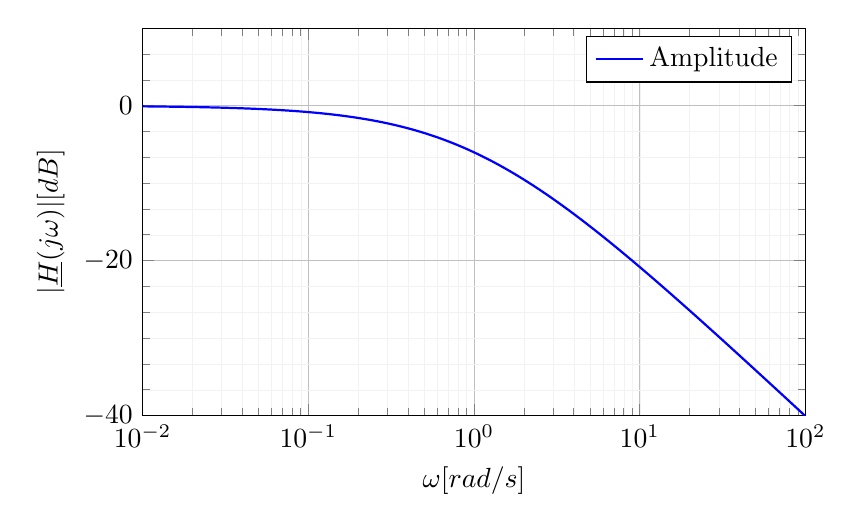
\begin{tikzpicture}
        \begin{semilogxaxis}[
            xlabel={$\omega [rad/s]$},
            ylabel={$|\underline{H}(j\omega)|[dB]$},
            xmin=0.01, xmax=100,
            ymin=-40, ymax=10,
            xmode=log,
            grid=both,
            grid style={line width=.1pt, draw=gray!10},
            major grid style={line width=.2pt,draw=gray!50},
            minor tick num=5,
            width=10cm,
            height=6.5cm,
            ]

            \addplot[domain=0.01:1000, blue, thick, samples = 1000] {
                20 * log10(1/(1+x))
            };
            \addlegendentry{Amplitude};
        \end{semilogxaxis}
    \end{tikzpicture}
\end{center}
\textbf{Phasengang:}
\begin{center}
    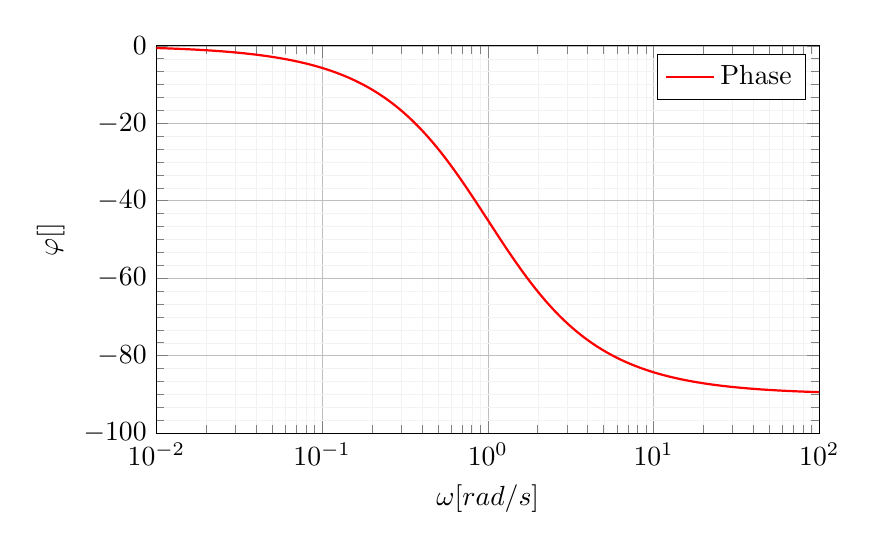
\begin{tikzpicture}
        \begin{semilogxaxis}[
                xlabel={$\omega [rad/s]$},
                ylabel={$\varphi [\degree]$},
                xmin=0.01, xmax=100,
                ymin=-100, ymax=0,
                xmode=log,
                grid=both,
                grid style={line width=.1pt, draw=gray!10},
                major grid style={line width=.2pt,draw=gray!50},
                minor tick num=5,
                width=10cm,
                height=6.5cm,
            ]

            \addplot[domain=0.01:100, red, thick, samples = 1000] {-atan(x/1)};

            \addlegendentry{Phase};

        \end{semilogxaxis}
    \end{tikzpicture}
\end{center}
\subsection{Umrechnen rad/s nach Hz}

Die Kreisfrequenz \( \omega \) wird in Einheiten Radiant pro Sekunde (\(
\text{rad/s} \)) angegeben und beschreibt, wie schnell sich ein periodisches
Signal pro Sekunde vollständig umkreist oder vollständig durchläuft. \\ Die
Frequenz \( f \) wird in Hertz (\( \text{Hz} \)) gemessen und gibt an, wie oft
sich ein periodisches Signal innerhalb einer Sekunde wiederholt oder wie viele
vollständige Zyklen es pro Sekunde durchläuft. \\ Die Umrechnung zwischen \(
\omega \) und \( f \) erfolgt durch folgende Formel:

\[
    \omega = 2 \pi f
\]
\\
Umrechnung von \( f \) zu \( \omega \)
\[
    f = \frac{\omega}{2 \pi}
\]

\section{Filter}
\subsection{Grenzfrequenz}
Die Grenzfrequnez bezeichnet die Frequenz, bei der ein Filter anfängt, Signale
zu beeinflussen oder zu verändern.
\begin{itemize}

    \item \textbf{Definition:} Die Grenzfrequenz bei Filter 1. Ordnung ist bei 3 dB definiert, an diesem Punkt ist das Ausgangssignal im Vergleich zum Eingangssignal um 3 dB abgeschwächt. 3 dB entspricht $\sqrt{\frac{1}{2}} = \frac{1}{\sqrt{2}} = 0,7071$. Das entspricht 70,71\% der Eingangsspannung. Bei Filter 2.Ordnung ist diese bei 6dB.
    \item \textbf{Bandbreite:} Die Bandbreite eines Filters ist zwischen den beiden 3-dB-Punkten definiert.

    \item \textbf{Phase:} Bei Filtern erster Ordnung beträgt die Phasenverschiebung bei der Grenzfrequenz 45 Grad. Zweiter Ordnung beträgt die Phasenverschiebung 90 Grad

\end{itemize}
\newpage
\subsection{Tiefpass}
Ein Tiefpassfilter lässt Signale mit niedrigen Frequenzen passieren, während
hohe Frequenzen blockiert werden. Filter 1.Ordnung können durch LR- oder
RC-Glieder aufgebaut werden. Zweiter Ordnung mit einem LC-Glied. \\\\
\textbf{RC-Glied}
\begin{center}
    \begin{circuitikz}
        \draw (0,0) to[R=$R$] (2,0);
        \draw (2,0) to[C=$C$] (2,-1.5);
        \draw (0,-1.5) -- (3,-1.5);
        \draw (2,0) -- (3,0);
        \draw[->,blue,>=latex,fill=blue] (0,-0.25) -- (0,-1.25) node[midway, left,blue] {${U}_e$};
        \draw[->,blue,>=latex,fill=blue] (3,-0.25) -- (3,-1.25) node[midway, right,blue] {${U}_a$};
        \draw[black,fill=black] (2,0) circle (1.5pt);
        \draw[black,fill=black] (2,-1.5) circle (1.5pt);
        \draw[black] (0,0) circle (1.5pt);
        \draw[black] (0,-1.5) circle (1.5pt);
        \draw[black] (3,0) circle (1.5pt);
        \draw[black] (3,-1.5) circle (1.5pt);
    \end{circuitikz}
\end{center}

Bei niedrigen Frequenzen verhält sich der Kondensator wie ein Leerlauf, was bedeutet, dass die Ausgangsspannung $U_a$ die gleiche Spannung wie die Eingangsspannung $U_e$ aufweist.
Bei hohen Frequenz wird der Kondensator jedoch zu einem Kurzschluss, dieses bedeutet das am Ausgang das kein Spannung anliegt.\\\\
Übertragungsfunktion:

\[ \underline{H}(j\omega) = \frac{\underline{U_{a}}(j\omega)}{\underline{U_{e}}(j\omega)}=\frac{X_{C}}{R+X_{C}}=\frac{\frac{1}{j \omega C}}{R+\frac{1}{j \omega C}}=\frac{1}{1+j\omega R C}\]

Betrag der Übertragungsfunktion:

\[|\underline{H}(\omega)|=\frac{1}{\sqrt{1+(\omega C R)^2}}\]

Berechnung Grenzfrequenz:

\[ f_{g} = \frac{1}{2\pi RC} \]
\\
\textbf{LR-Glied}
\begin{center}
    \begin{circuitikz}
        \ctikzset{inductors/scale=1, inductor=american}
        \draw (0,0) to[L=$L$] (2,0);
        \draw (2,0) to[R=$R$] (2,-1.5);
        \draw (0,-1.5) -- (3,-1.5);
        \draw (2,0) -- (3,0);
        \draw[->,blue,>=latex,fill=blue] (0,-0.25) -- (0,-1.25) node[midway, left,blue] {${U}_e$};
        \draw[->,blue,>=latex,fill=blue] (3,-0.25) -- (3,-1.25) node[midway, right,blue] {${U}_a$};
        \draw[black,fill=black] (2,0) circle (1.5pt);
        \draw[black,fill=black] (2,-1.5) circle (1.5pt);
        \draw[black] (0,0) circle (1.5pt);
        \draw[black] (0,-1.5) circle (1.5pt);
        \draw[black] (3,0) circle (1.5pt);
        \draw[black] (3,-1.5) circle (1.5pt);
    \end{circuitikz}
\end{center}
Bei niedrigen Frequenzen verhält sich die Spule wie ein Kurzschluss, was bedeutet, dass die Ausgangsspannung $U_a$ die gleiche Spannung wie die Eingangsspannung $U_e$ aufweist.
Bei hohen Frequenz wird die Spule jedoch zu einem Leerlauf, dieses bedeutet das am Ausgang das kein Spannung anliegt.\\\\
Übertragungsfunktion:

\[ \underline{H}(j\omega) = \frac{\underline{U_{a}}(j\omega)}{\underline{U_{e}}(j\omega)}=\frac{R}{X_{L}+R}=\frac{R}{j\omega L+R}=\frac{1}{1+\frac{j\omega L}{R}}\]
Betrag der Übertragungsfunktion:

\[|\underline{H}(\omega)|=\frac{1}{\sqrt{1+(\frac{\omega L}{R})^2}}\]
Berechnung Grenzfrequenz:

\[ f_{g} = \frac{R}{2\pi L} \]

\textbf{LC-Glied}
\begin{center}
    \begin{circuitikz}
        \ctikzset{inductors/scale=1, inductor=american}
        \draw (0,0) to[L=$L$] (2,0);
        \draw (2,0) to[C=$C$] (2,-1.5);
        \draw (0,-1.5) -- (3,-1.5);
        \draw (2,0) -- (3,0);
        \draw[->,blue,>=latex,fill=blue] (0,-0.25) -- (0,-1.25) node[midway, left,blue] {${U}_e$};
        \draw[->,blue,>=latex,fill=blue] (3,-0.25) -- (3,-1.25) node[midway, right,blue] {${U}_a$};
        \draw[black,fill=black] (2,0) circle (1.5pt);
        \draw[black,fill=black] (2,-1.5) circle (1.5pt);
        \draw[black] (0,0) circle (1.5pt);
        \draw[black] (0,-1.5) circle (1.5pt);
        \draw[black] (3,0) circle (1.5pt);
        \draw[black] (3,-1.5) circle (1.5pt);
    \end{circuitikz}
\end{center}

Übertragungsfunktion:

\[ \underline{H}(j\omega) = \frac{\underline{U_{a}}(j\omega)}{\underline{U_{e}}(j\omega)}=\frac{X_{C}}{X_{L}+X_{C}}=\frac{\frac{1}{j\omega C}}{j\omega L+\frac{1}{j\omega C}}=\frac{1}{1-\omega^2 LC}\]
Betrag der Übertragungsfunktion:

\[|\underline{H}(\omega)|=\frac{1}{1+\omega^2 LC}\]

Berechnung Grenzfrequenz:

\[ f_{g} = \frac{1}{2\pi \sqrt{LC}} \]
\\
\textbf{Amplitudengang:}
\begin{center}
    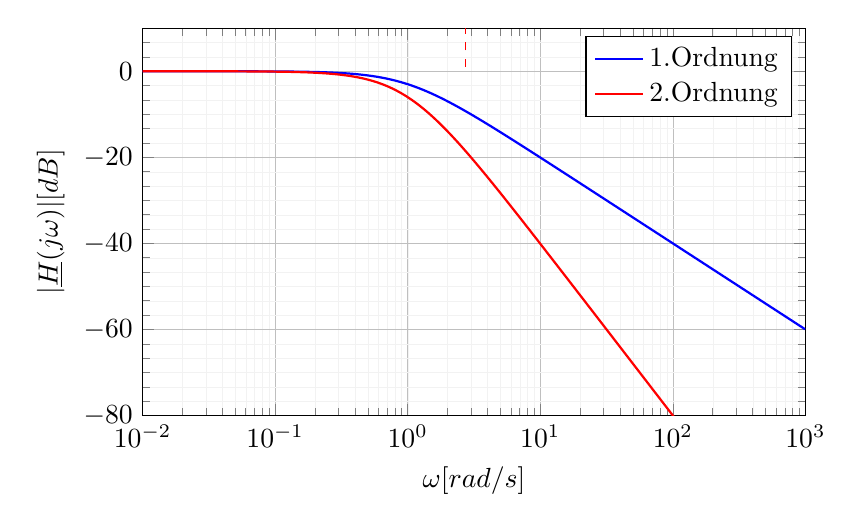
\begin{tikzpicture}
        \begin{semilogxaxis}[
            xlabel={$\omega [rad/s]$},
            ylabel={$|\underline{H}(j\omega)|[dB]$},
            xmin=0.01, xmax=1000,
            ymin=-80, ymax=10,
            xmode=log,
            grid=both,
            grid style={line width=.1pt, draw=gray!10},
            major grid style={line width=.2pt,draw=gray!50},
            minor tick num=5,
            width=10cm,
            height=6.5cm,
            ]

            \addplot[domain=0.01:1000, blue, thick, samples = 1000] {
                20 * log10(1/sqrt(1+(x)^2))
            };
            \addplot[domain=0.01:1000, red, thick, samples = 1000] {
                20 * log10(1/(1+x^2))
            };
            \addlegendentry{1.Ordnung};
            \addlegendentry{2.Ordnung};

            \draw[dashed, red] (0,1) -- (0,118) node[red,above] {$\omega_{\text{g}}$};


        \end{semilogxaxis}
    \end{tikzpicture}
\end{center}
\textbf{Phasengang:}
\begin{center}
    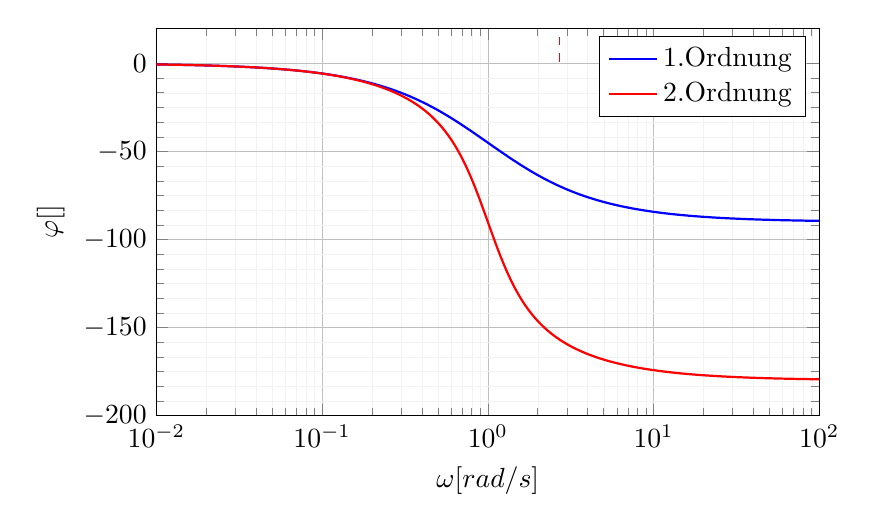
\begin{tikzpicture}
        \begin{semilogxaxis}[
                xlabel={$\omega [rad/s]$},
                ylabel={$\varphi [\degree]$},
                xmin=0.01, xmax=100,
                ymin=-200, ymax=20,
                xmode=log,
                grid=both,
                grid style={line width=.1pt, draw=gray!10},
                major grid style={line width=.2pt,draw=gray!50},
                minor tick num=5,
                width=10cm,
                height=6.5cm,
            ]

            \addplot[domain=0.01:1000, blue, thick, samples = 1000] {-atan(x/1)};
            \addplot[domain=0.01:1000, red, thick, samples = 1000] {-atan(x-(1/x))-90};

            \draw[dashed, red] (0,1) -- (0,180) node[red,above] {$\omega_{\text{g}}$};


            \addlegendentry{1.Ordnung};
            \addlegendentry{2.Ordnung};

        \end{semilogxaxis}
    \end{tikzpicture}
\end{center}
\newpage
\subsection{Hochpass}
Ein Hochpassfilter lässt nur Signale mit hohen Frequenzen passieren und
blockiert niedrige Frequenzen. Filter erster Ordnung können mit RC- oder
RL-Gliedern realisiert werden. Zweiter Ordnung mit einem LC-Glied.\\\\
\textbf{RC-Glied}
\begin{center}
    \begin{circuitikz}
        \draw (2,0) to[R=$R$] (2,-1.5);
        \draw (0,0) to[C=$C$] (2,0);
        \draw (0,-1.5) -- (3,-1.5);
        \draw (2,0) -- (3,0);
        \draw[->,blue,>=latex,fill=blue] (0,-0.25) -- (0,-1.25) node[midway, left,blue] {$U_{\text{e}}$};
        \draw[->,blue,>=latex,fill=blue] (3,-0.25) -- (3,-1.25) node[midway, right,blue] {$U_{\text{a}}$};
        \draw[black,fill=black] (2,0) circle (1.5pt);
        \draw[black,fill=black] (2,-1.5) circle (1.5pt);
        \draw[black] (0,0) circle (1.5pt);
        \draw[black] (0,-1.5) circle (1.5pt);
        \draw[black] (3,0) circle (1.5pt);
        \draw[black] (3,-1.5) circle (1.5pt);
    \end{circuitikz}
\end{center}
Übertragungsfunktion:

\[ \underline{H}(j\omega) = \frac{\underline{U_{a}}(j\omega)}{\underline{U_{e}}(j\omega)}=\frac{R}{X_{C}+R}=\frac{R}{\frac{1}{j \omega C}+R}=\frac{1}{1+\frac{1}{j\omega R C}}\]
Betrag der Übertragungsfunktion:

\[|\underline{H}(\omega)|=\frac{1}{\sqrt{1+(\frac{1}{\omega R C})^2}}\]
Berechnung Grenzfrequenz:

\[ f_{g} = \frac{1}{2\pi RC} \]
\\
\textbf{RL-Glied}
\begin{center}
    \begin{circuitikz}
        \ctikzset{inductors/scale=1, inductor=american}
        \draw (0,0) to[R=$R$] (2,0);
        \draw (2,0) to[L=$L$] (2,-1.5);
        \draw (0,-1.5) -- (3,-1.5);
        \draw (2,0) -- (3,0);
        \draw[->,blue,>=latex,fill=blue] (0,-0.25) -- (0,-1.25) node[midway, left,blue] {${U}_e$};
        \draw[->,blue,>=latex,fill=blue] (3,-0.25) -- (3,-1.25) node[midway, right,blue] {${U}_a$};
        \draw[black,fill=black] (2,0) circle (1.5pt);
        \draw[black,fill=black] (2,-1.5) circle (1.5pt);
        \draw[black] (0,0) circle (1.5pt);
        \draw[black] (0,-1.5) circle (1.5pt);
        \draw[black] (3,0) circle (1.5pt);
        \draw[black] (3,-1.5) circle (1.5pt);
    \end{circuitikz}
\end{center}
Übertragungsfunktion:

\[ \underline{H}(j\omega) = \frac{\underline{U_{a}}(j\omega)}{\underline{U_{e}}(j\omega)}=\frac{X_{L}}{R+X_{L}}=\frac{j \omega L}{R+j \omega L}=\frac{1}{1+\frac{R}{j\omega L}}\]

Betrag der Übertragungsfunktion:

\[|\underline{H}(\omega)|=\frac{1}{\sqrt{1+(\frac{R}{\omega L})^2}}\]

Berechnung Grenzfrequenz:

\[ f_{g} = \frac{R}{2\pi L} \]

\textbf{LC-Glied}
\begin{center}
    \begin{circuitikz}
        \ctikzset{inductors/scale=1, inductor=american}
        \draw (0,0) to[C=$C$] (2,0);
        \draw (2,0) to[L=$L$] (2,-1.5);
        \draw (0,-1.5) -- (3,-1.5);
        \draw (2,0) -- (3,0);
        \draw[->,blue,>=latex,fill=blue] (0,-0.25) -- (0,-1.25) node[midway, left,blue] {${U}_e$};
        \draw[->,blue,>=latex,fill=blue] (3,-0.25) -- (3,-1.25) node[midway, right,blue] {${U}_a$};
        \draw[black,fill=black] (2,0) circle (1.5pt);
        \draw[black,fill=black] (2,-1.5) circle (1.5pt);
        \draw[black] (0,0) circle (1.5pt);
        \draw[black] (0,-1.5) circle (1.5pt);
        \draw[black] (3,0) circle (1.5pt);
        \draw[black] (3,-1.5) circle (1.5pt);
    \end{circuitikz}
\end{center}
Übertragungsfunktion:

\[ \underline{H}(j\omega) = \frac{\underline{U_{a}}(j\omega)}{\underline{U_{e}}(j\omega)}=\frac{X_{L}}{X_{C}+X_{L}}=\frac{j \omega L}{\frac{1}{j \omega C}+j \omega L}=-\frac{\omega^2 LC}{1-\omega^2 LC}\]
Betrag der Übertragungsfunktion:

\[|\underline{H}(\omega)|=\frac{\omega^2 LC}{1+\omega^2 LC}\]

Berechnung Grenzfrequenz:

\[ f_{g} = \frac{1}{2\pi \sqrt{LC}} \]
\\
\textbf{Amplitudengang:}
\begin{center}
    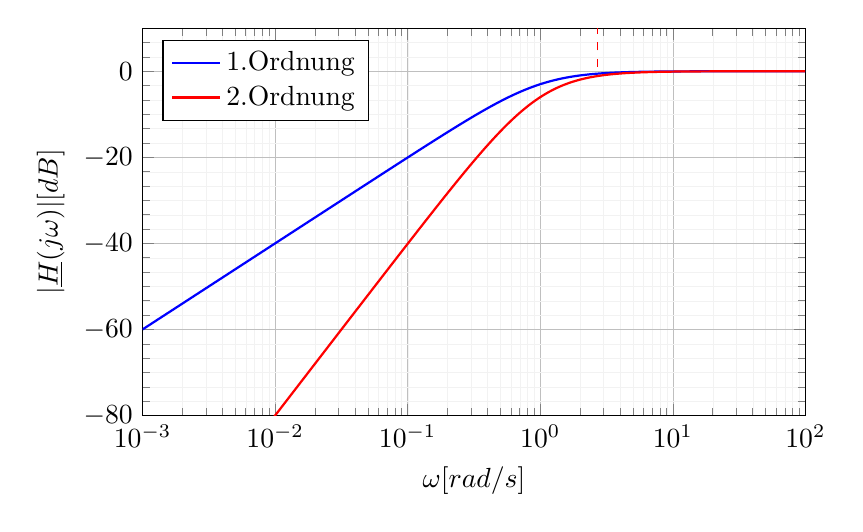
\begin{tikzpicture}
        \begin{semilogxaxis}[
            xlabel={$\omega [rad/s]$},
            ylabel={$|\underline{H}(j\omega)|[dB]$},
            xmin=0.001, xmax=100,
            ymin=-80, ymax=10,
            xmode=log,
            grid=both,
            grid style={line width=.1pt, draw=gray!10},
            major grid style={line width=.2pt,draw=gray!50},
            minor tick num=5,
            width=10cm,
            height=6.5cm,
            legend style={at={(0.03,0.97)},anchor=north west}
            ]

            \addplot[domain=0.001:100, blue, thick, samples = 1000] {
                20 * log10(1/sqrt(1+(1/x)^2))
            };
            \addplot[domain=0.001:100, red, thick, samples = 1000] {
                20 * log10(x^2/(1+x^2))
            };
            \draw[dashed, red] (0,1) -- (0,118) node[red,above] {$\omega_{\text{g}}$};
            \addlegendentry{1.Ordnung};
            \addlegendentry{2.Ordnung};
        \end{semilogxaxis}
    \end{tikzpicture}
\end{center}
\textbf{Phasengang:}
\begin{center}
    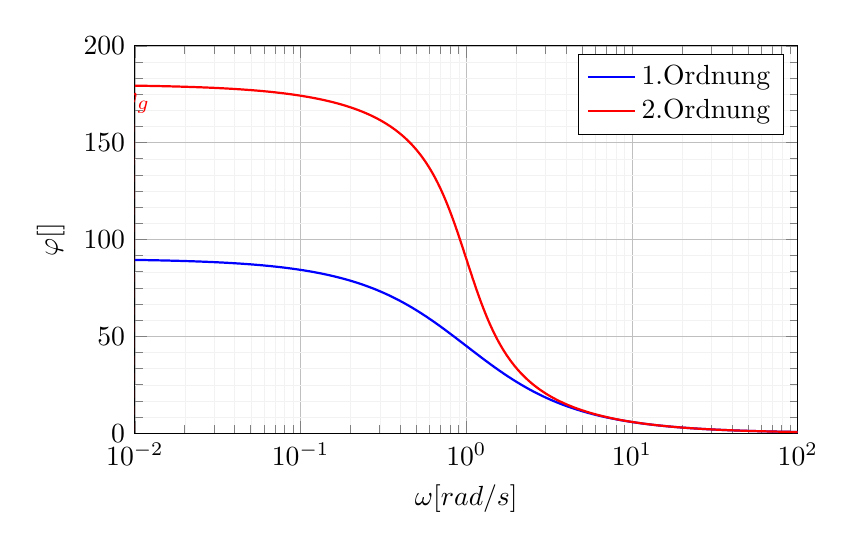
\begin{tikzpicture}
        \begin{semilogxaxis}[
                xlabel={$\omega [rad/s]$},
                ylabel={$\varphi [\degree]$},
                xmin=0.01, xmax=100,
                ymin=0, ymax=200,
                xmode=log,
                grid=both,
                grid style={line width=.1pt, draw=gray!10},
                major grid style={line width=.2pt,draw=gray!50},
                minor tick num=5,
                width=10cm,
                height=6.5cm,
            ]
            \addplot[domain=0.01:100, blue, thick, samples = 1000] {atan(1/x)};
            \addplot[domain=0.01:100, red, thick, samples = 1000] {atan(1/x-x)+90};
            \draw[dashed, red] (0.01,1) -- (0.01,160) node[red,above] {$\omega_{\text{g}}$};
            \addlegendentry{1.Ordnung};
            \addlegendentry{2.Ordnung};

        \end{semilogxaxis}
    \end{tikzpicture}
\end{center}

\subsection{Bandpass}
Ein Bandpassfilter lässt nur Signale innerhalb eines bestimmten
Frequenzbereichs passieren und blockiert Signale außerhalb dieses Bereichs.
Filter 1.Ordnung können durch RC-Netzwerk aufgebaut werden. 
Dieses kann durch einen Hochpassfilter und Tiefpassfilter aufgebaut werden.
\\\\
\textbf{RC-Netzwerk}
\begin{center}
    \begin{circuitikz}
        \draw (2.25,0) to[C=$C_{T}$] (2.25,-1.5);
        \draw (0,0) to[R=$R_{T}$] (2.25,0);
        \draw (2.25,0) to[C=$C_{H}$] (4,0);
        \draw (4,0) to[R=$R_{H}$] (4,-1.5);
        \draw (4,0) -- (5,0);
        \draw (0,-1.5) -- (5,-1.5);
        \draw[->,blue,>=latex,fill=blue] (0,-0.25) -- (0,-1.25) node[midway, left,blue] {$U_{\text{e}}$};
        \draw[->,blue,>=latex,fill=blue] (5,-0.25) -- (5,-1.25) node[midway, right,blue] {$U_{\text{a}}$};
        \draw[black,fill=black] (2.25,0) circle (1.5pt);
        \draw[black,fill=black] (2.25,-1.5) circle (1.5pt);
        \draw[black,fill=black] (4,0) circle (1.5pt);
        \draw[black,fill=black] (4,-1.5) circle (1.5pt);
        \draw[black] (0,0) circle (1.5pt);
        \draw[black] (0,-1.5) circle (1.5pt);
        \draw[black] (5,0) circle (1.5pt);
        \draw[black] (5,-1.5) circle (1.5pt);
    \end{circuitikz}
\end{center}

Übertragungsfunktion:
\[ \mathbf{R_{T}=R_{H} / C_{T}=C_{H}:} \]

\[ \underline{H}(j\omega) = \frac{\underline{U_{a}}(j\omega)}{\underline{U_{e}}(j\omega)}= \frac{1}{3+j(\omega R C-\frac{1}{\omega R C})}\]

\[ \mathbf{R_{T}\neq R_{H} / C_{T}\neq C_{H}:}\]
\[ \underline{H}(j\omega) = \frac{\underline{U_{a}}(j\omega)}{\underline{U_{e}}(j\omega)}= \frac{1}{1+\frac{1}{j\omega R_{H}C_{H}}}+\frac{1}{1+j\omega R_{T}+C_{T}}\]


Betrag der Übertragungsfunktion:

\[ \mathbf{R_{T}=R_{H} / C_{T}=C_{H}:} \]
\[|\underline{H}(\omega)|=\frac{1}{\sqrt{9+(\omega RC-\frac{1}{\omega RC})^2}}\]

\[ \mathbf{R_{T}\neq R_{H} / C_{T}\neq C_{H}:}\]
\[|\underline{H}(\omega)|=\frac{1}{\sqrt{1+(\frac{1}{\omega R_{H} C_{H}})^2}}+\frac{1}{\sqrt{1+(\omega C_{T} R_{T})^2}}\]

Berechnung Grenzfrequenzen:

\[ f_{0} = \frac{1}{2\pi RC} \]
\[ f_{0} = \sqrt{f_{oben}\cdot f_{unten}} \]
\[ B= f_{oben}-f_{unten} \]
\newpage
\textbf{Amplitudengang:}
\begin{center}
    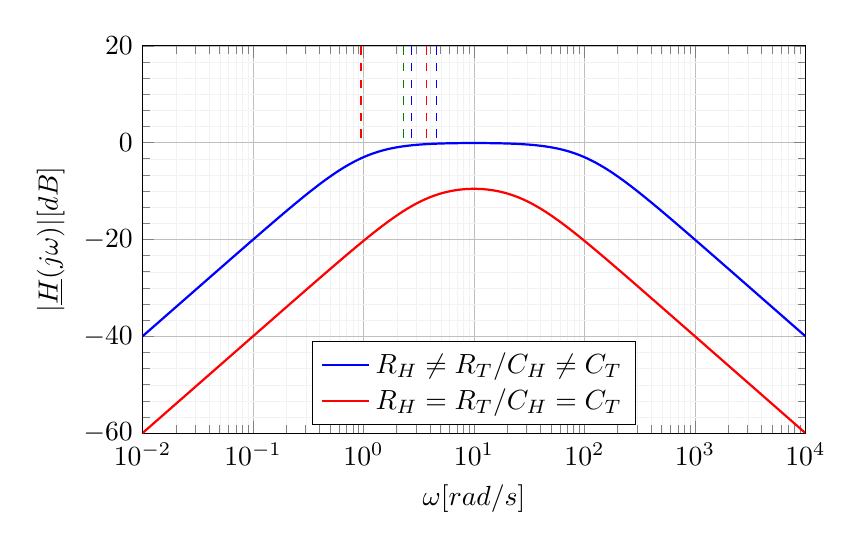
\begin{tikzpicture}
        \begin{semilogxaxis}[
            xlabel={$\omega [rad/s]$},
            ylabel={$|\underline{H}(j\omega)|[dB]$},
            xmin=0.01, xmax=10000,
            ymin=-60, ymax=20,
            xmode=log,
            grid=both,
            grid style={line width=.1pt, draw=gray!10},
            major grid style={line width=.2pt,draw=gray!50},
            minor tick num=5,
            width=10cm,
            height=6.5cm,
            legend style={at={(0.5,0.02)},anchor=south},
            ]

            \addplot[domain=0.01:10000, blue, thick, samples=1000] {20 * log10(1/sqrt(1+(1/(x))^2))+20*log10(1/sqrt(1+(0.01*x)^2))};


            \addplot[domain=0.001:10000, red, thick, samples = 1000] {
                20*log10(1/(sqrt(9+(x*0.1-(1/(x*0.1)))^2)))
            };

           
            \addlegendentry{$R_{H}\neq R_{T} / C_{H}\neq C_{T}$};
            \addlegendentry{$R_{H}=R_{T} / C_{H}=C_{T}$};
            \draw[dashed, green!50!black] (-4,704) -- (5,704);
            \draw[dashed, green!50!black] (-4,664) -- (5,664);
            \draw[green!50!black, <->] (-3.5,704) -- node[right,font=\footnotesize, green!50!black]{$\Delta 3dB$} (-3.5,664);

            \draw[dashed, blue] (0,1) -- (0,810) node[blue,above] {$\omega_{\text{unten}}$};
            \draw[dashed, blue] (4.6,1) -- (4.6, 810) node[above, blue] {$\omega_{\text{oben}}$};

            \draw[dashed, red] (0.95,1) -- (0.95,870) node[red,above] {$\omega_{\text{unten}}$};
            \draw[dashed, red] (3.7,1) -- (3.7, 870) node[above, red] {$\omega_{\text{oben}}$};
            \draw[dashed, green!50!black] (2.3,1) -- (2.3,840) node[green!50!black,above] {$\omega_{\text{0}}$};

        \end{semilogxaxis}
    \end{tikzpicture}
\end{center}
\textbf{Phasengang:}
\begin{center}
    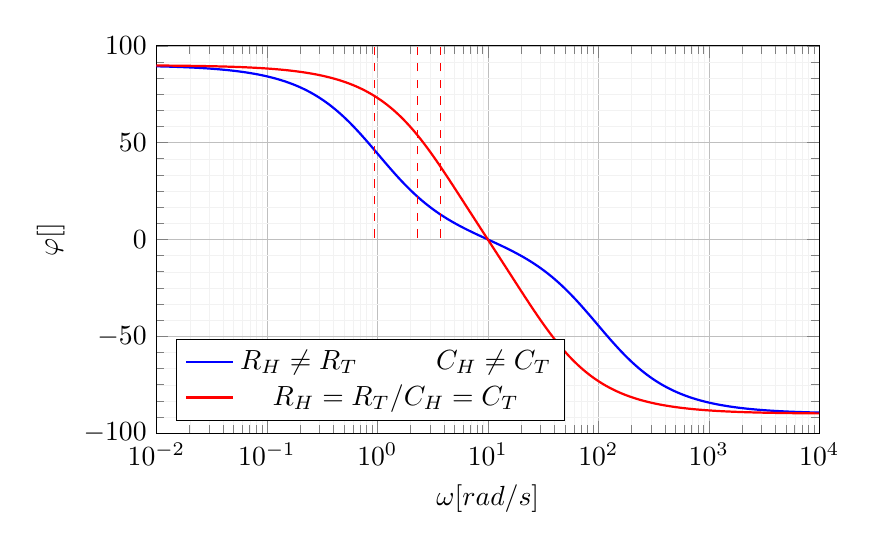
\begin{tikzpicture}
        \begin{semilogxaxis}[
                xlabel={$\omega [rad/s]$},
                ylabel={$\varphi [\degree]$},
                xmin=0.01, xmax=10000,
                ymin=-100, ymax=100,
                xmode=log,
                grid=both,
                grid style={line width=.1pt, draw=gray!10},
                major grid style={line width=.2pt,draw=gray!50},
                minor tick num=5,
                width=10cm,
                height=6.5cm,
                legend pos=south west,
            ]
            \addplot[domain=0.01:10000, blue, thick, samples=1000] 
            {-atan(x/1)+atan(1/(0.01*x))};


            \addplot[domain=0.01:10000, red, thick, samples = 1000] {
                %atan(1/x)-atan(x/100)
                -atan((1/3)*(x*0.1-(1/(x*0.1))))
            };

            \addlegendentry{$R_{H}\neq R_{T} \hspace{1cm} C_{H}\neq C_{T}$};
            \addlegendentry{$R_{H}=R_{T} / C_{H}=C_{T}$};
            \draw[dashed, red] (0.95,1) -- (0.95,170) node[red,above] {$\omega_{\text{unten}}$};
            \draw[dashed, red] (3.7,1) -- (3.7, 170) node[above, red] {$\omega_{\text{oben}}$};
            \draw[dashed, red] (2.3,1) -- (2.3,170) node[red,above] {$\omega_{\text{0}}$};

            \addlegendentry{Phase};

        \end{semilogxaxis}
    \end{tikzpicture}
\end{center}
\newpage
\subsection{Allpass / Phasenschieber}
Ein Allpassfilter lässt alle Frequenzen passieren, ändert jedoch die Phasenlage
der Signale, während die Amplituden unverändert bleiben.

\begin{center}
    \begin{circuitikz}
        \draw (0.5,1) to[R=$R1$] (2,1);
        \draw (2,1) -- (2.5,1);
        \draw (2.25,1) -- (2.25,0);
        \draw (0,0) -- (0.5,0);
        \draw (2.5,1) to[R=$R2$] (4,1);
        \draw (2.25,0) node[op amp, noinv input down, anchor=-]{\texttt{OPV}};
        \draw (0.5,1) -- (0.5,-0.98);
        \draw (0.5,-0.98) to[R=$R$] (2,-0.98);
        \draw (2,-0.98) -- (2.25,-0.98);
        \draw (2.25,-0.98) to[C=$C$] (2.25,-2.48);
        \draw (0,-2.48) -- (5,-2.48);
        \draw (4,1) -- (4.64,1);
        \draw (4.64,1) -- (4.64,-0.49);
        \draw (4.64,-0.49) -- (5,-0.49);
        \draw[->,blue,>=latex,fill=blue] (0,-0.25) -- (0,-2.23) node[midway, left,blue] {$U_{\text{e}}$};
        \draw[->,blue,>=latex,fill=blue] (5,-0.74) -- (5,-2.23) node[midway, right,blue] {$U_{\text{a}}$};
        \draw[black,fill=black] (2.25,1) circle (1.5pt);
        \draw[black,fill=black] (2.25,-0.98) circle (1.5pt);
        \draw[black,fill=black] (0.5,0) circle (1.5pt);
        \draw[black,fill=black] (4.64,-0.49) circle (1.5pt);
        \draw[black] (0,0) circle (1.5pt);
        \draw[black] (0,-2.48) circle (1.5pt);
        \draw[black] (5,-0.49) circle (1.5pt);
        \draw[black] (5,-2.48) circle (1.5pt);
    \end{circuitikz}
\end{center}
Übertragungsfunktion:
\[R_{1}=R_{2} \Rightarrow \text{Verstärkung}=\frac{R_{2}}{R_{1}}=1\]
\[ \underline{H}(j\omega) = \frac{\underline{U_{a}}(j\omega)}{\underline{U_{e}}(j\omega)}=\frac{2}{j \omega RC+1}-1=\frac{2-j\omega RC-1}{j\omega RC+1}=\frac{1-j\omega RC}{1+j\omega RC} \]
Betrag der Übertragungsfunktion:

\[|\underline{H}(\omega)|=\frac{1+j\omega RC}{1+j\omega RC}\]

Berechnung Grenzfrequenz:

\[ f_{g} = \frac{1}{2\pi RC} \]

\textbf{Amplitudengang:}
\begin{center}
    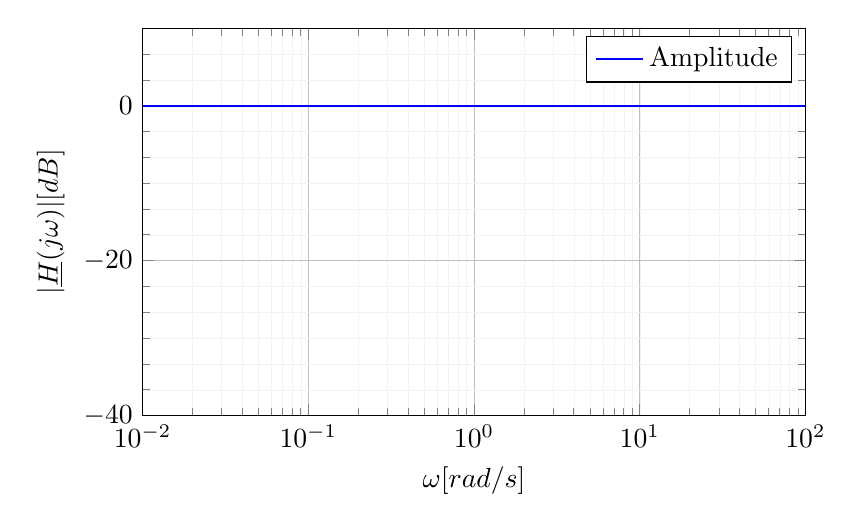
\begin{tikzpicture}
        \begin{semilogxaxis}[
            xlabel={$\omega [rad/s]$},
            ylabel={$|\underline{H}(j\omega)|[dB]$},
            xmin=0.01, xmax=100,
            ymin=-40, ymax=10,
            xmode=log,
            grid=both,
            grid style={line width=.1pt, draw=gray!10},
            major grid style={line width=.2pt,draw=gray!50},
            minor tick num=5,
            width=10cm,
            height=6.5cm,
            ]

            \addplot[domain=0.01:100, blue, thick, samples = 1000] {
                20 * log10(sqrt(1+(+x)^2)/sqrt(1+(x)^2))
                % 20 * log10(2)/(1+(x)^2))
            };
            \addlegendentry{Amplitude};
        \end{semilogxaxis}
    \end{tikzpicture}
\end{center}
\textbf{Phasengang:}
\begin{center}
    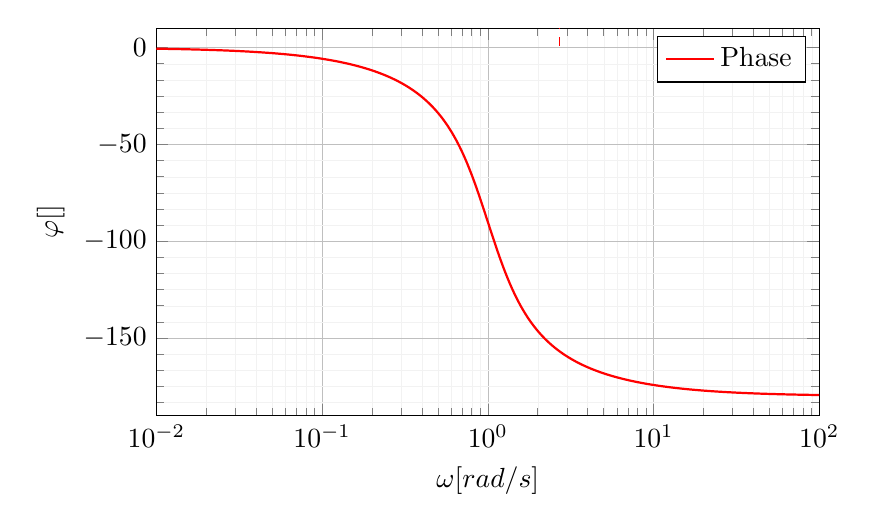
\begin{tikzpicture}
        \begin{semilogxaxis}[
                xlabel={$\omega [rad/s]$},
                ylabel={$\varphi [\degree]$},
                xmin=0.01, xmax=100,
                ymin=-190, ymax=10,
                xmode=log,
                grid=both,
                grid style={line width=.1pt, draw=gray!10},
                major grid style={line width=.2pt,draw=gray!50},
                minor tick num=5,
                width=10cm,
                height=6.5cm,
            ]
            \addplot[domain=0.01:100, red, thick, samples = 1000] {-atan(x-(1/x))-90};
            \addlegendentry{Phase};
            \draw[dashed, red] (0,1) -- (0,170) node[red,above] {$\omega_{g}$};

        \end{semilogxaxis}
    \end{tikzpicture}
\end{center}